\documentclass[a4paper,11pt]{article}
\usepackage[utf8]{inputenc}
\usepackage{textcomp}
\usepackage{lmodern}
\usepackage{listings}
\usepackage{graphicx}
\usepackage{listings}
\usepackage{color}
\definecolor{lightgray}{rgb}{0.9,0.9,0.9}
\definecolor{darkgray}{rgb}{0.4,0.4,0.4}
\definecolor{purple}{rgb}{0.65, 0.12, 0.82}
\usepackage{url}
\usepackage[top=3cm,bottom=3cm,left=3cm,right=3cm]{geometry}

\title{Royal Military Academy\\
	INFO-Y113 --- Management of Security: \\
	Concept Of Operations v2 \& Risk Analysis}

\author{DANHIER Pierre, LECOCQ Alexis, NYAKI Loïc}



\begin{document}
\maketitle
\vfill
Professor:  MEES Wim\\
Teacher Assistant: DEBATTY Thibault
\newpage
\tableofcontents

\newpage

\section{Introduction}
In recent years, cyber-security has become a primary concern for companies all over the world. No matter the size of the company, data often represent the heart of their business and whether the concern is the secrecy of intellectual property, or users' privacy, the theft of private data bears a huge cost for companies. Be it a cost in terms of money (lawsuits, fines) or reputation (loss of trust, public outrage). In the case of government agencies, states secrets and other classified information could be stolen by a foreign nation, possibly leading to the loss of lives in conflict zones, loss of political leverage on the international scene, domestic political turmoil and scandals or simply public embarrassment.\\

When trying to protect these sensitive data, a common measure is be to physically isolate the network from the internet, by creating an \textit{air gap}. Acting this way ensures that the data from the network is inaccessible from the outside world. The main issue with this method is that inevitably, some external data or files will at some point need to be imported into the secure network, be it for software update, or simply because some files from the outside are necessary for the people working in the secure network. In that case, a manual import (via USB drive, by connecting an external laptop into the secure network, or by using some other data transfer device) will be necessary.\\

The problem with that method is that it can compromise the security of the secure network. For instance, the data that is manually transferred into the network may have been infected by a malware, or the secure network might already be infected by a virus. In both cases, it could be possible for some malicious code to exfiltrate data, or to spread a virus outside, by secretly writing on the device that was originally used to import the data into the network, such as USB drives or laptops.\\

As a consequence, there is a need for a solution that prevents data leaks while allowing the transfer of files from an outside network into a secure network.

\section{Goals of the project}
\label{sec:goals}
Goals define the general direction of what the organization aims to accomplish, in the long term. Here, we wish to design a system that accomplishes three main goals :

\begin{enumerate}
\item{Create a device that completely prevents the exfiltration of data from a secure network, while allowing data to be transferred from the outside world into that secure network.}
\item{Ensure the availability of the system. The down times should be as minimum as possible.}
\item{Allow specific users to manage and monitor this system through an administration web page.}
\end{enumerate}

In this project, the general solution is imposed and should be a data diode, which will be described in section~\ref{sec:data-diode}.

\section{Scope}
It is important to precisely identify the scope of this project, in relation to our goals and objectives.\\

Our solution is destined to be integrated in an existing system. As such, when considering the security of the system as a whole, we must identify which security aspects fall under our responsibility and which don't. 

\subsection{In scope}
The following elements are in scope, which means that it is our responsibility to make sure that the security of these elements is ensured.

\begin{itemize}
\item{The availability of the service}
\item{The confidentiality of user data and credentials when interacting with the data diode (see section \ref{sec:data-diode})}
\item{The impossibility to exfiltrate data from the secure network through an interaction with the data-diode}
\item{The integrity of the data pushed through the data diode}
\end{itemize}

\subsection{Out of scope}
\label{sec:outscope}
The following elements are out of scope. This means that the security of these elements does not fall under our responsibility, but rather under the responsibility of the client, or another third party.

\begin{itemize}
\item{The physical access to the hardware, such as the power button or Ethernet cables}
\item{The securisation of the access to the data once they are stored in the database}
\item{The physical integrity of the hardware}
\item{The electrical power source}
\item{The security within the secure network, such as the presence of malwares or other viruses}
\item{The behaviour of the employees allowed to interact with the diode}
\end{itemize}


\section{Data Diode}
\label{sec:data-diode}
To ensure the integrity and the confidentiality of the data within our system and the availability of the service, we are going to implement a \textit{data diode}.\\

Just like an electrical diode only conduct electrical current in one direction, a data diode is a networking device that only allows data to flow in one direction. It is composed of two physical servers: one server communicates with the outside network and the other one communicate with the secure network. The two servers are to one another by a single unidirectional fiber optics cable.\\

A fiber optic connection normally uses two cables: one for each direction. In the case of 	 data diode, only one cable is used, allowing the data to flow in one direction. The cable going in the other direction is physically cut. As a consequence, data going through a data diode can only flow in one direction, which is one of the goals required in section \ref{sec:goals}.\\

The one-way communication channel between the two sides of the data-diode forbids the use of usual TCP based protocols (such as HTTP or FTP), as TCP requires bi-directional communication between two parties. As data between the two sides of the data-diode can only flow in one direction, we need data to be send over a protocol that doesn't require bi-directional communication. This can be done by using UDP for the communication between our two servers.\\

However UDP comes with its own limitations, as it doesn't ensure the order at which the paquets arrive, nor does it manage packets loss. These issues will therefore need to be taken into account at the software level.\\


\begin{figure}
%	\centering
%	\def\svgwidth{\columnwidth}
%	\input{img/system2.pdf_tex}
	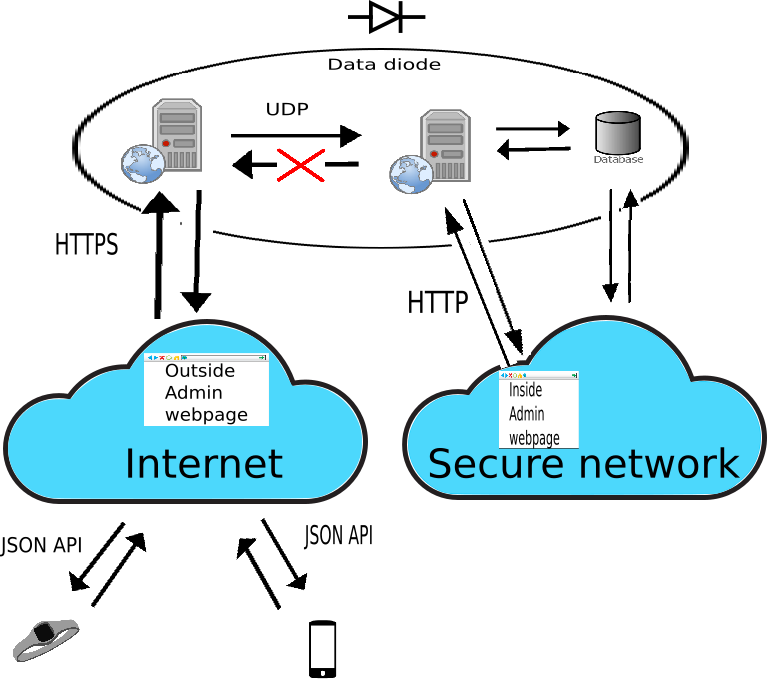
\includegraphics[scale=0.7]{img/system2.png}
	\caption{High level architecture of our data diode.}
\end{figure}


\subsection{Applications}
\subsubsection{JSON API}
We propose a JSON API to import files comming from connected devices to a secure network. To push data, a device needs to send a HTTP request to the outside machine with the basic authentication of the protocol in the headers and the JSON file in the body. When the request is received, the outside machine parse the HTTP request into a JSON file and send it with UDP to the secure side server. This machine will then store the file.

\subsubsection{Administration and User Management}
\label{sec:administration}
One of the goals of this project is the creation of a web interface to manage the data-diode. We will implement a web interface on the unsecure side that allows administrators to add new users or new administrators and a second web interface on the secure side that monitors the arrival of the UDP packets and creates an access to the data.

\subsubsection{Mockups}
\textbf{Unsecure side webpage}
\begin{center}
\begin{tabular}{cc}
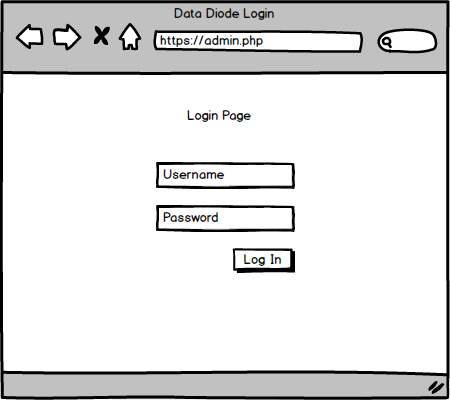
\includegraphics[scale=0.5]{img/outsideLogin.png} & 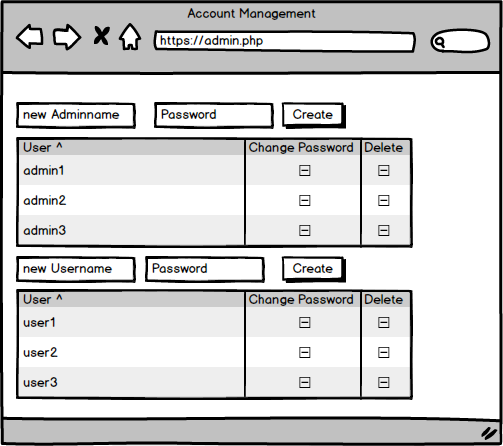
\includegraphics[scale=0.45]{img/outsideManagement.png}\\
\end{tabular}
\end{center} 

\textbf{Secure side webpage}
\begin{center}
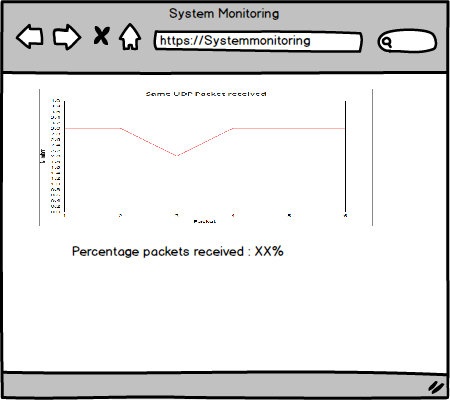
\includegraphics[scale=0.5]{img/linkudp.png}
\end{center}



\subsection{Physical Architecture}
The data-diode is composed of two separate servers connected to each other through a unidirectional fiber optics cable. The server facing the outside network is called \textit{the sender}, the server facing the secure network is called \textit{the receiver}.\\

Each server contains the following components :
\begin{itemize}
\item{Two network interfaces: one for connecting to a network, and one for connecting to the other server}
\item{A fiber optic adapter, to translate the signal coming from the fiber optic cable from light into a signal that can be transmitted through an Ethernet port.}
\end{itemize}

\subsection{Software architecture}
The data-diode is composed of two servers, \textit{the sender} and \textit{the receiver}, which have different roles. 

\subsubsection{The Sender}
The \textit{sender} must be able to receive HTTP requests from the outside network and to transmit JSON files to the \textit{receiver} via UDP.\\

The sender must therefore be comprised of :
\begin{itemize}
\item{A UDP client}
\item{A web server}
\item{A php server}
\end{itemize} 

\subsubsection{The Receiver}
The \textit{receiver} must be able to receive UDP paquets and reconstruct them as a JSON file that will be placed in a database. \\

In summary, the receiver will contain :
\begin{itemize}
\item{A UDP server}
\item{A web server}
\item{A php server}
\item{A MYSQL database}
\end{itemize}

\section{Users}
We identify two types of users : the administrators and the simple users.

\subsection{Simple Users}
Simple users are the data pushers using their connected devices.
\subsection{Administrators}
The role of the administrators is to manage the users and other administrators .
\section{Administration and Management}
\subsection{Administration of Simple Users}
Administrators can create and delete user accounts. If a user lost his password, he needs to contact an administrator who will give him a new one.

\subsection{Administration of other Administrators}
Administrators are able to create an administrator account, or to suspend the account of another administrator.

\subsection{Data diode Installation and Configuration}
At first use, the data diode automatically runs all its programs with default values. Each relevant value, such as IP address or open ports can be modified manually in a configuration file.

\subsubsection{Installation}
The data-diode is provided to the client with the programs already installed, and a default administrator account. At first use, the password needs to be modified.\\

The machine works with the default IP address \textbf{192.168.1.1}. The IP can be later changed manually.

\subsubsection{Configuration}
The data-diode settings will be specified in a configuration file that can be modified manually.


\section{Risk analysis}
In this section, we assess risk and describe how to manage it. This implies identifying threat sources, the components (or resources) as well as the potential impact that an attack on a component would have.

\subsection{Threat sources}
Threat sources describes the vectors through which an incident can happen. We identify the following threat sources:\\
\begin{itemize}
\item Malicious user: a user that would voluntarily use the system in a way such as to create problems 
\item Administrator mistake: an administrator that would make a mistake, such as launching the wrong command, or clicking on the wrong button
\item Malicious administrator: an administrator who would sabotage the system on purpose
\item Physical access: a person gaining physical access to the data-diode
\item System failure: a crash of the system
\item Malwares: various malware present on either the secure network, or public network
\item Zero Day Exploit: the exploitation of an unknown security flaw
\item The UDP protocol: this protocol doesn't ensure that packets arrive in the correct order, or that they arrive at all
\end{itemize}
\subsection{Components}
The components are the ressources that we are trying to protect inside of our system. We want to prevent an opponent to steal, corrupt or destroy any of the client's assets.
\subsubsection{Hardware components}
There is only one data-diode. However, it is composed of the three following hardware components:

\begin{itemize}
\item The sender
\item The receiver
\item The optical fiber between the two machines
\end{itemize}

\subsubsection{Software components}
The software components are all the programs that are necessary to the proper functioning of the data-diode. We identify the following elements:
\begin{itemize}
\item The inside administration webpage
\item The outside administration webpage
\item The php and web servers
\item The UDP client and server
\item The databases
\end{itemize}

\subsubsection{Information}
This section identifies the type of information that needs to be protected. We identify the following information:

\begin{itemize}
\item The user and administrator credentials
\item The data pushed through the diode
\end{itemize}
\subsection{Risk severity}
We define here the severity for each components of the CIA triad. Our numbers are indicators depending on activity of the clients.
\subsubsection{Confidentiality}
The confidentiality is the ability to protect the user/administrator credentials and the pushed data from beeing stolen by an opponent.\\
Here is our severity estimation for the lack of confidentiality:
\begin{itemize}
\item More than one user credentials $\rightarrow$ Medium
\item One or more administrator credentials $\rightarrow$ Major
\end{itemize}
\subsubsection{Integrity}
The integrity of our system is the insurance that the data pushed to our diode is not corrupted by the process.\\

Severity of corrupted packets:
\begin{itemize}
\item Less than 1 \% of corrupted or lost packets $\rightarrow$ Moderate
\item More than 1 \% of corrupted or lost packets $\rightarrow$ Major
\end{itemize}
\subsubsection{Availability}
Severity of downtimes:
\begin{itemize}
\item Less than 10 minutes $\rightarrow$ Minor
\item More than 10 minutes $\rightarrow$ Moderate
\item More than 1 hour $\rightarrow$ Major
\item More than 6 hour $\rightarrow$ Extreme
\end{itemize}
\subsection{Threats Assessments}
Here we define the risks incurred by our system relative to the CIA triad ( Confidentiality, Integrity and Availability). When several of these components are threatened, we keep the maximum impact as the general impact of the risk.
\subsubsection{Risk 1: Packet sniffing on the diode (admin) }
\textbf{Source} \\A malicious person has a physical access to the data diode\\
\textbf{Components} \\The data diode and the users database\\
\textbf{Description}\\ This person uses packet sniffing techniques on the unsecure sides of the data diode to obtain the credentials of an administrator. \\
\textbf{Impact}\\
With an administrator access the opponent can modify users and other adminstrators accounts. The confidentiality of the accounts is then corrupted.\\
\begin{center}

\begin{tabular}{|c|c|c|}
\hline
\textbf{Confidentiality} & \textbf{Integrity} & \textbf{Availability} \\
\hline
Major & None & None \\
\hline
\end{tabular}\\
\end{center}
\textbf{Likelihood}\\ As we recommand our client to protect the access to the diode, we assume that this risk is unlikely.\\
\textbf{Risk level}\\Medium\\

\subsubsection{Risk 2: Packet sniffing on the diode (user) }
\textbf{Source} \\A malicious person has a physical access to the data diode\\
\textbf{Component} \\The database\\
\textbf{Description}\\ This person uses packet sniffing techniques on the unsecure sides of the data diode to obtain the credentials of an user. \\
\textbf{Impact}\\
With user access the opponent can send data that we cannot be sure of the integrity. These data could corrupt the database informations.\\
\begin{center}

\begin{tabular}{|c|c|c|}
\hline
\textbf{Confidentiality} & \textbf{Integrity} & \textbf{Availability} \\
\hline
Medium & Major & None \\
\hline
\end{tabular}\\
\end{center}
\textbf{Likelihood}\\ As we recommand our client to protect the access to the diode, we assume that this risk is unlikely.\\
\textbf{Risk level}\\Medium\\


\subsubsection{Risk 3 : Shut down of the data diode }
\textbf{Source} \\A malicious person has a physical access to the data diode\\
\textbf{Component} \\The inside and outside machines\\
\textbf{Description}\\ This person can turn off the data diode. \\
\textbf{Impact}\\
The shut down of the diode cause a downtime of less than 30 minutes.\\
\begin{center}
\begin{tabular}{|c|c|c|}
\hline
\textbf{Confidentiality} & \textbf{Integrity} & \textbf{Availability} \\
\hline
None & None & Moderate \\
\hline
\end{tabular}\\
\end{center}
\textbf{Likelihood}\\ As we recommand our client to protect the access to the diode, we assume that this risk is unlikely.\\
\textbf{Risk level}\\Low\\

\subsubsection{Risk 4 : Optical fiber cut }
\textbf{Source} \\A malicious person has a physical access to the data diode\\
\textbf{Component} \\The connection between our two machines\\
\textbf{Description}\\ This person can cut the optical fiber between our two servers. \\
\textbf{Impact}\\
The shut down of the diode cause a downtime of about one hour if the client has the optical fiber piece in stock. The down time can be much larger if the client needs to order the piece.\\
\begin{center}
\begin{tabular}{|c|c|c|}
\hline
\textbf{Confidentiality} & \textbf{Integrity} & \textbf{Availability} \\
\hline
None & None & Extreme \\
\hline
\end{tabular}\\
\end{center}
\textbf{Likelihood}\\ As we recommand our client to protect the access to the diode and to have at least one optical fiber in stock, we assume that this risk is unlikely.\\
\textbf{Risk level}\\Medium\\

\subsubsection{Risk 5 : Deterioration of the data diode }
\textbf{Source} \\A malicious person has a physical access to the data diode\\
\textbf{Component} \\The whole data diode\\
\textbf{Description}\\ This person can damage or even destroy the data diode.  \\
\textbf{Impact}\\
Physical damage or complete destruction of the diode will obviously lead to a device replacement creating a several hours or days downtime.\\
\begin{center}
\begin{tabular}{|c|c|c|}
\hline
\textbf{Confidentiality} & \textbf{Integrity} & \textbf{Availability} \\
\hline
None & None & Extreme \\
\hline
\end{tabular}\\
\end{center}
\textbf{Likelihood}\\ As we recommand our client to protect the access to the diode, we assume that this risk is unlikely.\\
\textbf{Risk level}\\Medium\\

\subsubsection{Risk 6 : Flooding of the sender }
\textbf{Source} \\A malicious user send a lot of files in the goal of overloading the sender\\
\textbf{Component} \\The sender server\\
\textbf{Description}\\ The user will overload the system with data pushes. 
\\
\textbf{Impact}\\
 If this person can send more files that the system can handle, our system can become unavailable for several tens of minutes. \\
 \begin{center}
\begin{tabular}{|c|c|c|}
\hline
\textbf{Confidentiality} & \textbf{Integrity} & \textbf{Availability} \\
\hline
None & None & Moderate \\
\hline
\end{tabular}\\
\end{center}
\textbf{Likelihood}\\ This kind of attack is really popular and easy to make so the event is likely to occur.\\
\textbf{Risk level}\\Medium\\

\subsubsection{Risk 7 : Flooding of the outside webpage}
\textbf{Source} \\Knowing the IP address of our sender server,a malicious person sends a lot of connection requests to the unsecure side login webpage . \\
\textbf{Component} \\The outside webpage\\
\textbf{Description}\\ The outside administration webpage can be overloaded. \\
\textbf{Impact}\\
With an sufficient overload of this system, the administration webpage can be unavailable for several tens of minutes.\\
\begin{center}
\begin{tabular}{|c|c|c|}
\hline
\textbf{Confidentiality} & \textbf{Integrity} & \textbf{Availability} \\
\hline
None & None & Moderate \\
\hline
\end{tabular}\\
\end{center}
\textbf{Likelihood}\\ This kind of attack is really popular and easy to make so the event is likely to occur.\\
\textbf{Risk level}\\Medium\\

\subsubsection{Risk 8 : Brute force on the outside webpage }
\textbf{Source} \\A malicious user tries to obtain administrator rights.\\
\textbf{Component} \\The outside webpage\\
\textbf{Description}\\This malicious user can use brute force techniques or dictionnary attacks to find an administrator account. \\
\textbf{Impact}\\
This kind of attacks generate a lot of connection attemps. This overload on the webpage can lead to a several minutes downtime. If this attack succeed the user has the ability to modify other user or even administrator accounts. He also can delete all the user accounts so that the system cannot import data anymore.\\
\begin{center}
\begin{tabular}{|c|c|c|}
\hline
\textbf{Confidentiality} & \textbf{Integrity} & \textbf{Availability} \\
\hline
Major & None & Major \\
\hline
\end{tabular}\\
\end{center}
\textbf{Likelihood}\\ This kind of attack is really popular and easy to make so the event is likely to occur.\\
\textbf{Risk level}\\High\\

\subsubsection{Risk 9 : SQL injection on the outside webpage }
\textbf{Source} \\A malicious user tries to connect as an administrator without authorization.\\
\textbf{Component} \\The outside webpage\\
\textbf{Description}\\This person can use SQL injection in the login page in the goal of being connected as an administrator. \\
\textbf{Impact}\\
The user has the ability to modify other user or even administrators accounts. He also can delete all the user accounts so that the system cannot import data anymore.\\
\begin{center}
\begin{tabular}{|c|c|c|}
\hline
\textbf{Confidentiality} & \textbf{Integrity} & \textbf{Availability} \\
\hline
Major & None & Major \\
\hline
\end{tabular}\\
\end{center}
\textbf{Likelihood}\\ This kind of attack is really popular and easy to make so the event is likely to occur.\\
\textbf{Risk level}\\High\\

\subsubsection{Risk 10 : UDP packet loss }
\textbf{Source} \\UDP is not a secure protocol \\
\textbf{Component} \\The UDP connection between our 2 servers\\
\textbf{Description}\\As UDP is not a secure protocol, some packets can be lost between our two servers. Without ACK mecanism, the protocol does not allow us to know if we lost a packet. \\
\textbf{Impact}\\
The loss of a UDP packet can lead to uncorrect data.\\
\begin{center}
\begin{tabular}{|c|c|c|}
\hline
\textbf{Confidentiality} & \textbf{Integrity} & \textbf{Availability} \\
\hline
None & Moderate & None \\
\hline
\end{tabular}\\
\end{center}
\textbf{Likelihood}\\ With a so small optical fiber, this event is unlikely to occur.\\
\textbf{Risk level}\\Medium\\

\subsubsection{Risk 11 : UDP corrupted packet}
\textbf{Source} \\UDP is not a secure protocol \\
\textbf{Component} \\The UDP connection between our 2 servers\\
\textbf{Description}\\As UDP is not a secure protocol, a UDP packet can be corrupted but we have no way to ask it again because there is no ACK mecanism in UDP. \\
\textbf{Impact}\\
The corruption of a UDP packet can lead to uncorrect data.\\
\begin{center}
\begin{tabular}{|c|c|c|}
\hline
\textbf{Confidentiality} & \textbf{Integrity} & \textbf{Availability} \\
\hline
None & Moderate & None \\
\hline
\end{tabular}\\
\end{center}
\textbf{Likelihood}\\ With a so small optical fiber, this event is unlikely to occur.\\
\textbf{Risk level}\\Medium\\

\subsubsection{Risk 12 : Deletion of user accounts }
\textbf{Source} \\A malicious administrator wants to block the import of data.\\
\textbf{Component} \\The outside management webpage\\
\textbf{Description}\\This administrator can delete all the user accounts \\
\textbf{Impact}\\
Without any authorized user, the system cannot import data anymore. This can create a several hours downtime. \\
\begin{center}
\begin{tabular}{|c|c|c|}
\hline
\textbf{Confidentiality} & \textbf{Integrity} & \textbf{Availability} \\
\hline
None & None & Extreme \\
\hline
\end{tabular}\\
\end{center}
\textbf{Likelihood}\\ Having a malicious administrator is unlikely to occur.\\
\textbf{Risk level}\\Medium\\

\subsubsection{Risk 13 : Deletion of administrator accounts }
\textbf{Source} \\A malicious administrator wants to block user management.\\
\textbf{Component} \\The outside management webpage\\
\textbf{Description}\\This administrator can delete all the other administrator accounts \\
\textbf{Impact}\\
Without any other administrator, we cannot manage the users anymore.\\
\begin{center}
\begin{tabular}{|c|c|c|}
\hline
\textbf{Confidentiality} & \textbf{Integrity} & \textbf{Availability} \\
\hline
Major & None & Extreme \\
\hline
\end{tabular}\\
\end{center}
\textbf{Likelihood}\\ Having a malicious administrator is unlikely to occur.\\
\textbf{Risk level}\\Medium\\

\subsubsection{Risk 14 : CSRF in the outside webpage}
\textbf{Source} \\A malicious user wants to modify the users or administrators accounts.\\
\textbf{Component} \\The outside management webpage\\
\textbf{Description}\\This malicious user forges a request so that an administrator session is used to modify accounts.   \\
\textbf{Impact}\\
With this technique, the user can create an administrator account for himself or modify other accounts. He can then block the import of the data to the secure network. \\
\begin{center}
\begin{tabular}{|c|c|c|}
\hline
\textbf{Confidentiality} & \textbf{Integrity} & \textbf{Availability} \\
\hline
None & None & Major \\
\hline
\end{tabular}\\
\end{center}
\textbf{Likelihood}\\The opponent needs the unawareness of an administrator to lauch this attack. This event is then unlikely to occur.\\
\textbf{Risk level}\\Medium\\

\subsubsection{Risk 15 : Malware inside the secure side}
\textbf{Source} \\The secure network is infected by a malware.\\
\textbf{Components} \\The inside machine and the database.\\
\textbf{Description}\\This malware could flood the inside machine with http requests or encrypt the database.  \\
\textbf{Impact}\\
The flood of http request to the inside machine can create a several tens of minutes downtime and the encryption on the database can lead to a several hours downtime with a lack of integrity.\\
\begin{center}
\begin{tabular}{|c|c|c|}
\hline
\textbf{Confidentiality} & \textbf{Integrity} & \textbf{Availability} \\
\hline
None & Major & Extreme \\
\hline
\end{tabular}\\
\end{center}
\textbf{Likelihood}\\Since the access to the inside network is supposed to be protected by the client, we assume that this risk is unlikely.\\
\textbf{Risk level}\\Medium\\





\subsection{Summary}
\begin{tabular}{|c|c|c|c|c|}
\hline
Threat & Source & Impact& Likelihood & Evaluation \\
\hline
1 &  Packet sniffing (admin) & Major  & Unlikely & Medium\\
\hline
2 &  Packet sniffing (user)  & Major  & Unlikely & Medium\\
\hline
3 & Shut down of diode & Moderate & Unlikely & Low \\
\hline
4 &  Optical fiber cut & Extreme  & Unlikely & Medium\\
\hline
5 & Deterioration of the diode & Extreme & Unlikely & Medium\\
\hline
6 & Flooding the sender & Moderate & Likely & Medium\\
\hline
7 & Flooding on outside webpage & Moderate & Likely & Medium \\
\hline 
8 &  Brute Force on outside webpage & Major & Likely & High\\
\hline
9 & SQL injection on outside webpage & Major & Likely & High \\
\hline
10 & UDP packet loss & Moderate & Unlikely & Medium \\
\hline
11 & UDP corrupted packet & Moderate & Unlikely & Medium \\
\hline
12 & Deletion of user accounts & Extreme & Unlikely & Medium \\
\hline
13 & Deletion of administrator accounts & Extrele & Unlikely & Medium \\
\hline
14 & CSRF on the outside webpage & Major & Unlikely & Medium \\
\hline
15 & Malware in the secure network & Extreme & Unlikely & Medium \\
\hline

  
\end{tabular}
\subsection{Countermeasures}
\label{sec:countermeasures}
As security has a significative price for a company, we assume that low risks should be accepted.
\subsubsection{Risk 1 : Packet sniffing on the diode (admin) }
As the physical access to the diode is out of our scope, we transfer this risk to the client.
\subsubsection{Risk 2 : Packet sniffing on the diode (user) }
As the physical access to the diode is out of our scope, we transfer this risk to the client.
\subsubsection{Risk 3 : Shut down of the diode}
As the physical access to the diode is out of our scope, we transfer this risk to the client.
\subsubsection{Risk 4 : Optical fiber cut}
As the physical access to the diode is out of our scope, we transfer this risk to the client.
\subsubsection{Risk 5 : Deterioration of the data diode}
As the physical access to the diode is out of our scope, we transfer this risk to the client.
\subsubsection{Risk 6 : Denial of service attack through data flooding}
We mitigate this risk by limiting the amount of data that a user can send in a define time.
\subsubsection{Risk 7 : Flooding of the outside webpage}
We mitigate this risk by temporary blocking the opponent's IP adress when whe detect that the amount of failed connection attemps is too big to just be an administrator mistake.
\subsubsection{Risk 8 : Brute force on outside webpage}
We mitigate this risk by forcing users to have a password that respects some security criteria. The passwords should:

\begin{itemize}
	\item{Be 8 characters long, or more}
	\item{Contain at least one uppercase letter}
	\item{Contain at least one special character}
\end{itemize}

This restriction on passwords maximizes the size of the search space that will need to be bruteforced.

\subsubsection{Risk 9 : SQL injection on outside webpage}
We avoid this risk by using prepared statement mecanism on the login inputs.
\subsubsection{Risk 10 : UDP packet loss}
We mitigate this risk by pushing 3 times each UDP packets. We then only need one received packet over the three to obtain the data on the secure side.As the chance to have one lost packet is small, the probabilities to have 3 lost packets are nearly null.
\subsubsection{Risk 11 : UDP corrupted packet}
We mitigate this risk with the same techniques than for lost packets but including the UDP checksum. We only need one correct packet over the three to obtain the data on the secure side. The chances to have three corrupted packets are also nearly null.
\subsubsection{Risk 12 : Deletion of user accounts}
As the behaviour and the good will of the employees are under the responsability of the client, we transfer this risk to them.
\subsubsection{Risk 13 : Deletion of administrator accounts}
As the behaviour and the good will of the employees are under the responsability of the client, we transfer this risk to them.
\subsubsection{Risk 14 : CSRF on outside webpage}
We mitigate this risk by using tokens in the URL. When an administrator is connected to the administration webpage, a random token is attributed to him and this token will be needed in every request to the website.
\subsubsection{Risk 15 : Malware inside the secure side}
Since the security inside the secure network is out of our scope, we transfer this risk to the client.

\subsection{Residual risks}
\subsubsection{Risk 6 : Flooding on the outside webpage}
If the opponent uses a botnet with enough different IP adresses, he can DDoS attack our system with success.

\section{Implementation}
\label{sec:implementation}
The data diode is composed of two physical servers, called the \textit{sender} and the \textit{receiver}, each having two Ethernet network interfaces.\\

The first network interface is used to connect to the other server, using a unidirectional fiber optics cable. The second interface is used to connect to the secure network, or the outside network.

\subsection{Architecture}
\subsubsection{Sender}
The \textit{sender} is the server of the data-diode that is facing the outside network. It's mission is to push data to the server on the other side of the data-diode, called the \textit{receiver}.

\paragraph{Software}
The sender runs the following software:
\begin{itemize}
	\item{Operating system: Ubuntu server 16.04}
	\item{HTTP server: Nginx, listening on port \textit{80}}
	\item{UDP client: sends the data to the other side of the data-diode}
\end{itemize}

\subsubsection{Receiver}
The \textit{receiver} is the server of the data-diode that is facing the secure network. It listens to UDP messages, and stores them in a database. It's default IP address is \textbf{192.168.1.1}.


\paragraph{Software}
The receiver runs the following software:
\begin{itemize}
	\item{HTTP server, used for administration purpose}
	\item{UDP server: receives the data sent from the sender, on port \textbf{4242}}
	\item{Database : the receiver runs a MySql database, used for storing incoming messages. The database is listening on port \textbf{3306}}
\end{itemize}

\subsection{Countermeasures}
In section \ref{sec:countermeasures}, we described our choice of countermeasures to address risks. This section illustrates how these countermeasures were implemented.

\subsubsection{Denial of service attack through data flooding (Risk 6)}
We want to prevent a malicious user from sending an abnormal amount of data in an attempt to saturate the filesystem.\\

To mitigate this risk, we impose a limit on the amount of data that a user can send.


\subsubsection{Brute force attack on the outside web page (Risk 8)}
Only registered users can send data inside the secure network. However, an attacker could try to obtain a user password through a brute force attack. To mitigate this risk, users are required to use long passwords.

\subsubsection{SQL injection ou outside webpage (Risk9)}
Inserting data into a database is always a dangerous affair, due to the risk of SQL injection, where an attaquer will try to hide SQL code in the data he sends to the database.\\

A solid way to prevent this is the use of prepared statements. What follows is an example of how we use them:

\begin{lstlisting}[frame=single] 
function insert_data($data) {
  $sql = 'INSERT INTO data VALUES(?, ?, ?, ?, ?);';
  
  $params = array(
    $data['time'],
    $data['id'],
    1,
    $data['user'],
    json_encode($data['data']),
  );
  
  sql_request($sql, $params, $rows);
  
  return $rows;
}
\end{lstlisting}


\subsubsection{UDP packet loss (Risk 10)}
\label{sec:udp}
To mitigate the risk of packet loss, we send each packet several times. The number of times can be adjusted to the needs. In this case, we send each packet three times.

\begin{lstlisting}[caption={(sender/index.php) Each UDP packet is sent 3 times},captionpos=b]
  $repetition = 3
  $sock = udp_socket();
  for ($i = 0; $i < $repetition; $i++)
  {
    $r = socket_sendto($sock, $json, $len, null,
         $internal['ip'], $internal['port']);
    if ($r !== $len)
    {
      error('Error processing data (2).');
    }
  }
\end{lstlisting}

\subsubsection{UDP corrupted packets (Risk 11)}
The solution to packet corruption is the same as in section \ref{sec:udp}.

\subsubsection{CSRF attack on outside webpage (Risk 14)}
\textit{Cross-Site Request Forgery} (CSRF) is an attack that forces an end user to execute unwanted actions on a web application in which they're currently authenticated. This can compromise the entire application.\\

To mitigate this risk, we make use of CSRF token that is uniquely generated for each request.


\section{Demo Plan}
The previous section described how the the system will be eventually implemented. However, for the purpose of this demo, we are presenting a simplified version of the data-diode, where the physical machine has been simulated through software.\\

Instead of a physical data-diode, containing two servers connected to one another by a fiber optic cable, we use docker containers and some IP table manipulation.

\begin{lstlisting}[frame=single,caption={(start\_containers.sh) Creation of the containers, assignment of their IP addresses,setup of port bindings and connection to the networks.},captionpos=b] 
# Building container : inner side of the diode
cd internal/
docker build . -t diode_in-img

docker run -t -d --net secure-network --ip 10.0.0.2 -p 8880:80 
        --name diode-in 
        --cap-add=NET_ADMIN --cap-add=NET_RAW diode_in-img
cd -

# Building container : outter side of the diode
cd external/
docker build . -t diode_out-img 
docker run -t -d --net intra-diode --ip 192.168.0.3 
    -p 8881:80 -p 8882:443 
    --name diode-out diode_out-img
cd -

# Creating connecting a part of the diode to the outside, 
# and the other one to the inside
docker network connect --ip 192.168.0.2  intra-diode diode-in
docker network connect --ip 200.0.0.2 external-network diode-out
\end{lstlisting}

\subsection{Data-Diode servers}
The data-diode is composed of two servers. One facing towards the outside network, and one facing towards the inside network. We simulate these servers with docker containers, each having two virtual network interfaces.\\

Docker is a container technology that allows the execution of programs in an isolated environment. In our case, we use two containers that will represent the sender and the receiver.

\subsubsection{Docker Sender}
The sender container is responsible for pushing data from the outside of the data-diode into the inside.\\

The container was based on a Ubuntu image. However, as the docker Ubuntu image only contains the most important functionalities, many functionalities that are usually present on any Linux distributions are absent. Therefore, in order to create a container with the appropriate capabilities, the following packages needed to be installed:

\begin{itemize}
	\item{Nginx: The HTML server}
	\item{PHP 7.0: This was required to run our backend, which was implemented in PHP}
	\item{Net-tools: This package was required to be able to use the ifconfig command, and make sure that the network interface where properly initialized}
	\item{iputils-ping: This package installed the ping command}
	\item{makel: This package installs the Make automation tool}
	\item{vim: a text editor}
\end{itemize}

All these elements must be specified in a special configuration file called \textit{Dockerfile}. An excerpt of the file is displayed below :\\

\begin{table}
\lstinputlisting[firstline=1, lastline=28]{code/sender-Dockerfile}
\caption{An excerpt of the configuration file (Dockerfile) of the \textit{sender} container.}
\end{table}

\subsubsection{Docker Receiver}
The receiver container catches the messages sent by the \textit{sender}, and places them in a MySql database.\\

Similarly to the \textit{sender}, this container is based on a Ubuntu images. The following packages were also installed:

\begin{itemize}
	\item{Mysql-Server: A Mysql database}
	\item{Nginx: The HTML server}
	\item{PHP 7.0: This was required to run our backend, which was implemented in PHP}
	\item{PHP 7.0-mysql: PHP package required to interact with mysql}
	\item{Net-tools: This package was required to be able to use the ifconfig command, and make sure that the network interface where properly initialized}
	\item{iputils-ping: This package installed the ping command}
	\item{make: This package installs the Make automation tool}
	\item{vim: a text editor}
\end{itemize}

The configuration file (Dockerfile) of the \textit{receiver} is very similar to the Dockerfile of the \textit{sender} which is why it won't be displayed here. The full Dockerfile for the \textit{sender} and the \textit{receiver} can be found in appendix.

\subsection{Unidirectional Fiber optic}
\label{sec:unidirectional}
To simulate the fiber optic cable that has been cut, we use a script that modifies the IP table of the internal server.\\

The script, called \textit{fiber\_optic\_cut.sh}, drops all the paquets originating from the secure network that are trying to reach the \textit{intra-diode} network.\\

This script only contains the following command:\\

\begin{lstlisting}[frame=single,caption={(fiber\_optic\_cut.sh) All paquets going to the intra-diode network are dropped.},captionpos=b] 
iptables -A OUTPUT -d 192.168.0.0/24 -j DROP
\end{lstlisting}

which virtually cuts the connection between the \textit{receiver} and the \textit{sender}, by dropping all paquets going to the \textit{sender}.

\begin{figure}
	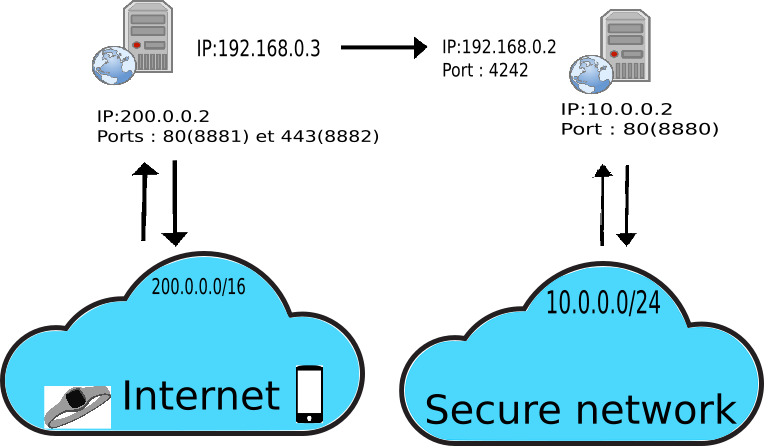
\includegraphics[scale=0.7]{img/reseau.png}
	\caption{High level architecture of our data diode.}
\end{figure}

\subsection{Networks}
Each container needs to placed in a network. More precisely, client containers are connected to a single network each, while server containers (diode-in, diode-out) are each connected to two network, as they are both at the edge of two networks.\\

In an effort to correctly simulate reality, we define three networks: The outside network, the intra-diode network, and the secure network.


\begin{table}
\lstinputlisting[firstline=1, lastline=28]{code/create_networks.sh}
\caption{(\textit{create\_networks.sh}) the scripts that creates the three docker networks.}
\end{table}

\subsubsection{Outside Network}
This network represents the outside, unsafe and insecure network. The subnet address range is \textbf{200.0.0.0/16}, and one of the two network interfaces of the \textit{sender} is connected to this network, with IP \textbf{200.0.0.2}.\\


We simulate a client initiating a connection to the \textit{sender}, from the outside network, by using a binding between port \textbf{80} from the sender container, and port \textbf{8881} from the host machine (in this case, the host machine is the laptop computer running docker).\\

We can then connect to the public side of the data-diode and access its web interface, through port \textbf{8881} on the host machine.

\subsubsection{Intra-Diode Network}
This network represents the inside of the data diode. It is only populated by two containers, which are the inner part and outer part of the data diode. Between these two servers, communication can only go from the outer part to the inner part, as mentioned in section \ref{sec:unidirectional}.\\

This network has a subnet of \textbf{192.168.0.0/24} and the sender and receiver are connected to that network with, respectively IP \textbf{192.168.0.3} and IP \textbf{192.168.0.2}.

\subsubsection{Secure Network}
This is the secure part of the system, the secure network. The innermost part of the data-diode is connected to this network, with the IP \textbf{10.0.0.2}. The receiver runs a web server on port \textbf{80}. It can be accessed from the secure network.\\

The network itself has the subnet \textbf{10.0.0.0/24}.

In our simulation, we connect to the webserver of the receiver through port \textbf{8880} of the host machine, thanks to a port binding between the receiver and the host..

\section{Conclusion}
The goal of this project was to make us demonstrate our ability to understand and formalize a problem leading to the creation of a fitting solution to that problem.\\

This was done in three steps. First, we showed that we understood the problem, through the creation of a document called \textit{Concept of OperationS} (CONOPS). We then identified the risks inherent to the system, and show how these risks could be managed, in a section called \textit{Risk Analysis}. Lastly, we specified a solution for a real implementation of the system  and presented a live demonstration of a prototype that embodied the result of the two previous steps.\\

The result was a functioning simulation of a data-diode that successfully implemented the goals of this project, as well as the risk countermeasures that were specified in the document.

\end{document}
